\begin{figure}[t]
  \centering
  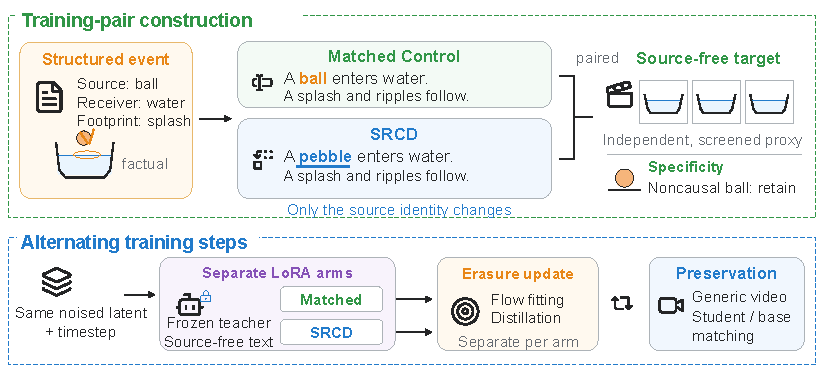
\includegraphics[width=\linewidth]{fig_task_method_overview.pdf}
  \caption{\textbf{Causal-role erasure and the source-slot intervention.}
  The schematic prompts differ only in factual source identity and share an
  independently generated, screened source-free video as a distributional proxy.
  Matched and \methodshort{} train separate mechanism-specific LoRA adapters
  with identical initialization, stochastic draws, objectives, and schedule.
  Both use the same frozen teacher conditioned on the source-free prompt;
  erasure updates strictly alternate with frozen-model matching on generic
  preservation videos. The noncausal ball denotes specificity evaluation,
  not hard-negative training data. Drawings illustrate the task and training
  design, not measured model outputs.}
  \label{fig:task-method-overview}
\end{figure}
